\documentclass{ociamthesis}         % Load document base.

\usepackage[utf8]{inputenc}         % Set .tex encoding (for pdfLaTeX).
\usepackage[T1]{fontenc}            % Set document font.

\usepackage[                        % Set default text spacing to 1.5
    onehalfspacing,                 % and allows to switch to 1.0 later
]{setspace}                         % on.

%%%%%%%%%%%%%%%%%%%%%%%%%%%%%%%%%%%%%%%%%%%%%%%%%%%%%%%%%%%%%%%%%%%%%%%%
%%%%%%%%%%%%%%%%%%%%%%%%% Recommended Imports %%%%%%%%%%%%%%%%%%%%%%%%%%%
%%%%%%%%%%%%%%%%%%%%%%%%%%%%%%%%%%%%%%%%%%%%%%%%%%%%%%%%%%%%%%%%%%%%%%%%

\usepackage{amssymb}                % Load American Mathematical Society
\usepackage{amsthm}                 % packages to enhance equations.
\usepackage{amsfonts}
\usepackage{amsmath}
\usepackage{mathtools}
\allowdisplaybreaks                 % Allow equations to break when to
                                    % long.

\usepackage{siunitx}                % Load SI unit support. Can be used
\sisetup{                           % to alignment units in tables and
  round-mode      = places,         % in general keep their format
  round-precision = 2,              % consistent. Here it is setup to 
}                                   % consistently round to two places.

\usepackage[hyphens]{url}           % Set URLs to hyperlinks and allow
                                    % to break them on hyphens (-).
                                    
\usepackage[                        % Make clickable hyperlink.
    hyperindex = true,              % Set TOC to be clickable.
    breaklinks = true,              % Allow links to break over lines.
]{hyperref}

\usepackage[all]{hypcap}            % Hyperlinks to captions link to the
                                    % correct place within the document.


\usepackage[english]{babel}         % Load language support. Use
                                    % "english" for English and
                                    % "ngerman" for German.

\usepackage[
    style        = numeric,
    autocite     = plain,
    sorting      = nyt,             % Sort by "name" "year "title"
    maxcitenames = 2,               % Set max number of cited authors.
    maxbibnames  = 10,              % Set max number of author names in
                                    % bibliography.
    backend      = biber,
]{biblatex}

\DefineBibliographyStrings{ngerman}{%          As babel switches 
    andothers = {et\addabbrvspace al\adddot} % "et al." to "u. a." we 
}                                   %          override this behavior
                                    %          back to "et al."
    

\addbibresource{references.bib}     % Load your bib from a file       
\addbibresource{zotero_references.bib}

\usepackage{xcolor}                 % Allows coloring of elements and
                                    % defining own colors.

\usepackage{graphicx}
\graphicspath{ {figures/} }         % Set the default path for graphics

\usepackage{caption}                % Allows to customize captions
                                    % further.

\usepackage{subcaption}             % Allows to customize subcaptions.
                                    % Relies on caption package.

\usepackage[english]{cleveref}      % Improves references so you don't
                                    % have to write "Chapter~\ref{}"
                                    % Instead use \cref{} and \Cref{}.
                                    % Use the same language option as
                                    % babel.

% \usepackage{nicefrac}             % Allows write fractions as ½

\usepackage{longtable} 	            % Allows tables in a longtable
                                    % environment to go over multiple
                                    % pages.

\usepackage{diagbox}                % Allows splitting a table cell
                                    % diagonally.

\usepackage{minted}                 % Load code highlighting package.
\usemintedstyle{tango}              % Set highlight color style.
\definecolor{background}{RGB}{      % Define code background color as
    250,                            % light gray.
    250,
    250,
}
\setminted{                         % Setup global minted config.
   linenos    = true,               % Use line numbers.
   numbersep  = 8pt,                % Set number distance.
   breaklines = true,               % Break long lines if possible.
   frame      = lines,              % Add a top and bottom frame line.
   bgcolor    = background,         % Set defined background color.
}


\usepackage{csquotes}               % Set quotes to be compatible with
                                    % biblatex.

\usepackage{datetime2}              % Package to handle timestamps.
\DTMsetup{useregional}              % Checking babels language setup
                                    % and format accordingly.


\usepackage[                        % Use glossaries.
    acronym,                        % Create special acronym glossary.
    toc                             % Include glossaries in toc.
]{glossaries}
\makeglossaries
\loadglsentries{                    % Load acronyms for acronym
    glossaries/acronyms.tex         % glossary.
}
\loadglsentries{                    % Load symbols for main
    glossaries/symbols.tex          % glossary.
}


\usepackage{lipsum}                 % Generates example text in
                                    % abstract. You can remove this.

\usepackage{algorithm}
\usepackage{algpseudocode}
\usepackage{nicefrac}


%%%%%%%%%%%%%%%%%%%%%%%%%%%%%%%%%%%%%%%%%%%%%%%%%%%%%%%%%%%%%%%%%%%%%%%%
%%%%%%%%%%%%%%%%%%%%%%%%% Cover Configuration %%%%%%%%%%%%%%%%%%%%%%%%%%
%%%%%%%%%%%%%%%%%%%%%%%%%%%%%%%%%%%%%%%%%%%%%%%%%%%%%%%%%%%%%%%%%%%%%%%%
\title{Text localization and recognition for scholarly videos}
\author{Anis Mekacher}
\matriculationnumber{10027832}
\department{Institut für Data Science -- Fachgebiet Visual Analytics}
\college{Leibniz Universität Hannover}
\logo{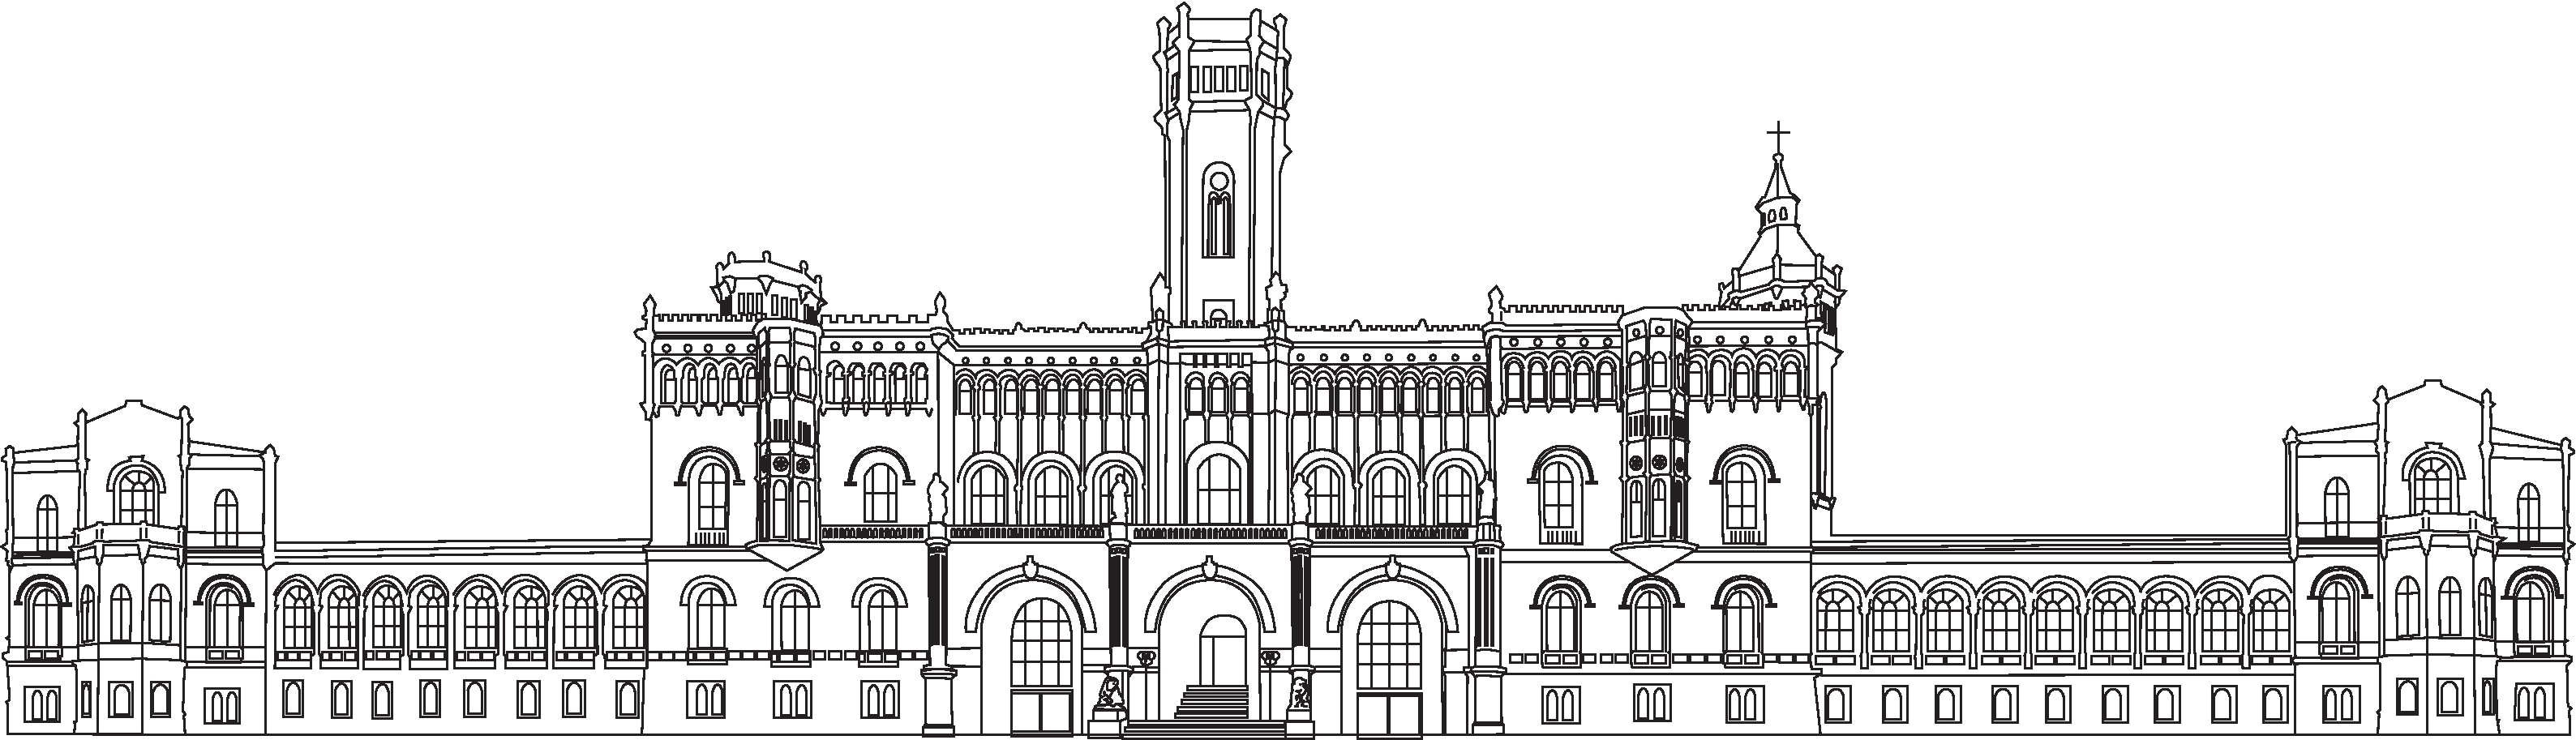
\includegraphics[width=120mm]{figures/welfen}}
\thesistype{Bachelorarbeit}
\degree{Bachelor of Science (B. Sc.)}
\degreedate{\DTMdate{2023-02-16}}
\firstexaminer{Prof. Dr. Ralph Ewerth}
\secondexaminer{Prof. Dr. Sören Auer}
\supervisor{M. Eng. Matthias Springstein}
\place{Hannover}
% \germancover                      % Include this to set the cover
                                    % to German instead of English.
                                    % Remember to also switch babel
                                    % and cleveref languages.


%%%%%%%%%%%%%%%%%%%%%%%%%%%%%%%%%%%%%%%%%%%%%%%%%%%%%%%%%%%%%%%%%%%%%%%%
%%%%%%%%%%%%%% end the preamble and start the document %%%%%%%%%%%%%%%%%
%%%%%%%%%%%%%%%%%%%%%%%%%%%%%%%%%%%%%%%%%%%%%%%%%%%%%%%%%%%%%%%%%%%%%%%%
\begin{document}
\pagenumbering{roman}               % Use roman page numbers.

\setcounter{secnumdepth}{3}         % Set the number of sectioning
\setcounter{tocdepth}{3}            % levels that get number and appear
                                    % in the contents.

\maketitle                          % Create a title page from the 
                                    % preamble info.

\chapter*{Abstract}
Education, like many other fields, has seen a massive move toward digitization, and this progress was amplified as the COVID-19 virus hit and all students were forced to attend online lectures. This sudden switch to online courses meant hundreds of hours of unlabeled video lectures got uploaded to online learning platforms. This thesis focuses on labeling these videos by extracting written text from videos. The extracted text can then be used to implement content-based search in lecture video datasets.     % Include abstract befor toc.

\tableofcontents                    % Print table of contents here.
\phantomsection                     % Add anchor for hyperref.
\addcontentsline{toc}{chapter}{     % Add list of tables as chapter to
        \listtablename              % the table of contents.
    }
\listoftables                       % Print list of tables here.
\phantomsection                     % Add anchor for hyperref.
\addcontentsline{toc}{chapter}{     % Add list of figures as chapter to
        \listfigurename             % the table of contents.
    }
\listoffigures                      % Print list of figures here.
\printglossary[type=\acronymtype]   % Print list of acronyms.
\printglossary                      % Print (default) list of symbols.
\cleardoublepage                    % Make sure new content is on
                                    % odd page
\pagenumbering{arabic}              % Switch page numbers to arabic.
\setcounter{page}{1}                % Reset page counter.

%%%%%%%%%%%%%%%%%%%%%%%%%%%%%%%%%%% % Include all your chapters

\chapter{Introduction}
\label{ch:intro}

Videos of lectures are a great learning resource for students as they give them the freedom to go back to any point in the course and restudy the material to clarify some questions, study for an exam, or reinforce their knowledge.
This reliance on lecture videos for learning has significantly increased in the last couple of years, especially after the COVID-19 pandemic hit and most students were forced to learn from home.
Online learning platforms like Stud-IP and TIB AV-Portal provide easy access to thousands of hours of recorded lectures that students can quickly and easily accessible at any time.
But the use cases for the recorded lectures are severely limited by the searchability of videos.

\section{Problems}
Most online learning platforms function more or less like a video database to which recordings of lectures get uploaded with minimal information about what the content is about and which topics are handled. The description of videos usually consists of a short title, which may be only the lecture number.

This limited description of content poses a problem for information retrieval systems which are usually text-based. Searching for a term can be based only on the given title or short description of the video, which doesn't provide enough information about the content to allow the measurement of document (video) heuristics like \gls{tf–idf}, thus resulting in unreliable search results.

One further problem of lecture videos is the inability to search for a term and jump to the specific location where it was mentioned, as is the case with PDF documents; for the student to find the point in time at which the term was written, they need to use the seek bar to slowly go through the video until they find the desired location.

These problems strongly limit the use of recordings as reference material for exam revision.

\section{Possible remediation of the problem}

Though the videos might not be well documented, information about their content can still be extracted from the videos themselves. The goal, in this case, is to turn the videos into a searchable format like text; this might be done either based on the contained audio using methods like Speech-To-Text or based on their frames (images) using \gls{ocr}.

\gls{ocr} is the process of transcribing still images to machine-readable text. It consists of two main tasks: text localization and text recognition, but it may include other image-processing tasks.


\gls{ocr} has been used extensively in:
\begin{itemize}
    \item Document digitization: a scanned page of a document/book gets transcribed to its ASCII equivalent
    \item Scene Text Recognition: extraction of text from scenes with complex backgrounds like in the case of autonomous vehicles.
    \item Image text translation: Text is detected and translated in real-time like in the Google Translate App
\end{itemize}

In the context of scholarly videos, \gls{ocr} may be used to extract text from video frames; this text can then be merged into a single block that represents the contents of the video.
This transcribed text can then be used in text-based information retrieval systems to improve the accuracy of the search results further.

\section{About this thesis}

This thesis focuses on improving \gls{ocr} specifically for use in scholarly videos.

Running \gls{ocr} on videos comes with certain challenges that define some of the goals I want to achieve in the thesis. Some of these problems are:
\begin{itemize}
    \item Videos are long and contain thousands of frames that need to be processed individually; for example, a one-hour thirty-minute video (the typical length of a lecture) recorded at 30 \gls{fps} contains $90 * 60 * 30 = 162000$ Frames that need to be processed. If processing one frame takes 100ms, this video will take four hours and thirty minutes which quickly becomes impractical when processing hundreds of lectures per day.
    So efficiency and speed are some goals this thesis tries to achieve.
    \item Falsely transcribed text (accuracy) or non-transcribed text (recall) can lead to erroneous results when used with information retrieval systems. So improving accuracy and recall is one of the goals we set to achieve.
    \item Videos may be shaky, blurry, far away, or have bad lighting; all factors directly affect the accuracy and recall of the transcribed text. So making the system reliable and robust to variations further increases the practical use of \gls{ocr} for video transcription.
\end{itemize}
\chapter{Related Work}
\label{ch:rw}

Since the explosion of deep learning methods with the publication of Alexnet in 2013, there have been numerous developments in text/object detection and text recognition techniques.

Until 2017 object detection was mainly based on region proposals. Region proposal methods, as the name suggests, propose a region of the input image to be scanned for the existence of a possible object. This technique was used by \gls{rcnn} \cite{girshick_rich_2014} (2014) and improved upon by Fast \gls{rcnn} \cite{girshick_fast_2015} (2015) and Faster \gls{rcnn} \cite{ren_faster_2017} (2016) with the introduction of Region Proposal Networks. Building on the improvements of Faster R-CNN, Mask R-CNN \cite{he_mask_2017} (2017) also detects objects in the image but based on pixel-wise masks instead of bounding boxes. \gls{panet} \cite{liu_path_2018} (2018) and \gls{psenet} \cite{wang_shape_2019} (2019) are two text detection models that improved on mask R-CNN using FPNs and extra post-processing algorithms. \gls{dbnet} \cite{liao_real-time_2019} (2019) is also very similar in architecture to PSENet but uses a dynamic binarization method when creating the binary masks for segmentation. This was further enhanced in \gls{dbnetpp} \cite{liao_real-time_2023} (2022) by adding an attention mechanism to merge of different scale feature maps from the Feature Pyramid Network. FourierNet \cite{riaz_fouriernet_2021} (2021) took another approach when representing the detection boxes and instead of using bounding box coordinates it uses a more compact Fourier series representation. All these methods were too slow because the same computations were applied multiple times to different proposed regions, making them inefficient. The \gls{yolo} method introduced in 2015 \cite{redmon_you_2016} solved these limitations by running the expensive convolutional layer computation only once and aggregating the results at the end. This model was then further developed into YOLOv2 (2016) \cite{redmon_yolo9000_2017}, YOLOv3 (2018) \cite{redmon_yolov3_2018}, YOLOv4 (2020) \cite{wang_scaled-yolov4_2021}, and YOLOv7 (2022) \cite{wang_yolov7_2022} with each newer version increasing the speed and accuracy of the model.

Before new deep-learning algorithms took off in 2013, traditional text recognition methods like tesseract \cite{smith_overview_2007} used different shape embedding techniques and classifiers like \gls{svm}s to recognize different characters in an image. But since 2013 most text recognition methods made use of deep-learning techniques like \gls{lstm} and \gls{cnn}s; \gls{sar} \cite{li_show_2019} (2019) is one of those models that used \gls{crnn} to recognize texts of arbitrary shapes. Although LSTMs are versatile they have a performance bottleneck as they can only process data sequentially. This problem has been remediated by the introduction of Transformers \cite{vaswani_attention_2017} in 2017 and since then most models were based on this architecture. \gls{nrtr} \cite{sheng_nrtr_2019} (2019) is one such model that combined transformer architecture and CNNs for feature embedding to recognize text efficiently. This was further improved by \gls{satrn} \cite{lee_recognizing_2020} (2020) to make the recognition more robust for arbitrarily shaped text.  \gls{master} \cite{lu_master_2021} (2021) replaced the encoder of the transformer with Global Context Network that spread the attention over the whole image not only on the local features. \gls{abinet} \cite{fang_read_2021} (2021) added an external language model to iteratively rectify incorrectly transcribed words by the transformer. The idea of enhancing the vision models with language models was taken a step further by \gls{parseq} \cite{bautista_scene_2022} (2022) by integrating the language model into the transformer decoder using a multi-modal learning approach.
\chapter{Foundations}
\chapter{Methology}

\section{Video processing pipeline}

To get the text transcription from a lecture video, most of the previously-stated problems need to be addressed at some point, which naturally leads to a multi-step processing pipeline.

\begin{figure}[H]
        \centering
        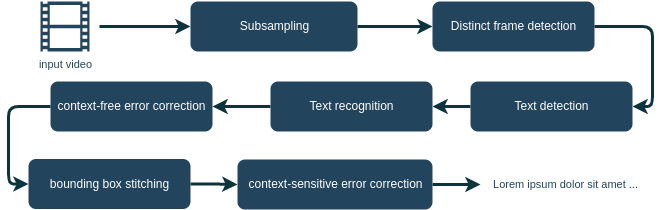
\includegraphics[width=140mm]{figures/ocr_pipeline}
        \caption{Video processing pipeline}
        \label{meth:ocr_pipeline}
\end{figure}

As shown in figure \ref{meth:ocr_pipeline}, the video processing pipeline contains seven steps that take an input video and output its transcription. First, the input video is subsampled to reduce the total number of frames that need to be processed; the selected frames are then fed to a distinct frame detection algorithm that finds the set of unique frames from the subsampled frames. After the distinct frame detection, all the images are processed separately and in parallel, so each frame first passes through a text detection model that puts bounding boxes around the text fields in the image; each bounding box is then cropped from the image and passed to a text recognition model that transcribes the text found in the image. The transcribed text is then passed to a context-free (dictionary-based) error correction algorithm to detect and fix some transcription errors. After error correction, we have a set of bounding boxes and their corresponding text per frame; on their own, they're independent words with no connection to one another and can serve as a video search index but to get a more comprehensive understanding of the text content, the words need to be turned back into complete sentences; that's why the next step is bounding box stitching (merging) which connects multiple bounding boxes into one to make up full sentences. The sentences can then be passed to a context-based error correction method to fix grammatical errors that could have been caused by incorrect transcription of some words.

In the following sections, we'll go into more detail about each step.

\section{Subsampling and distinct frame detection}

In the first step, the video file is read, and then a list of all the frames' indexes is returned; it's important at this point to focus on the fact that not the frames themselves are read into memory but only their corresponding ids, this is done to reduce the memory load as most lecture videos are pretty long and depending on the file format may be quite large. Additionally, we might also want to process multiple videos in parallel on the same machine, and we would run out of memory pretty fast if they all needed to be loaded into memory. We then choose how many frames per second of video we want to process, and based on the video's \gls{fps}, we determine how many frames should be skipped. The formula for this is  $\text{skip\_frames} = \text{video\_fps} \ / \ \text{target\_fps}$; so for a $30$ FPS video and chosen target FPS of $1$, we'll only consider every $30$th frame starting from $0$. Depending on the selected target FPS, this significantly reduces the number of frames that need to be processed by the later stages of the pipeline and thus makes inference run faster. Videos with 30+ FPS have frames that are taken $1s / 30 = 0.033s  = 33.33ms$ apart; for a fast-moving target, a lot can change in 33ms, but for still videos of lectures most frames that are taken in a second are identical.

In lecture videos, not a lot changes even when considering frames every second, and this is due to multiple reasons related to how lectures are usually constructed. In a typical lecture, the presenter either writes or displays a slide and then spends a considerable amount of time, ranging from seconds to minutes, explaining the material presented. Moreover, if the presenter is actively writing and not displaying already written materials, then a good portion of the time is spent writing the content on the board; from a text recognition pipeline's point of view, the frames that include the text being actively written are irrelevant, because the transcribed text from each frame would be a duplicate of the last one with none or some words added to it; that's why the only frame that matters is the final one with all the text written on it. That frame contains all the information about the previous ones that we actually care about; so we call it a distinct or unique frame and it's the one that gets processed by the rest of the pipeline.

As explained in \ref{ch:foundations:ocr_challenges}, state-of-the-art methods for distinct frame detection rely on encoding the individual frames to feature vector representations and then comparing two vectors based on cosine similarity or square difference. The used models for encoding are mainly object detection or recognition methods, which are heavy-duty, computationally expensive, and take a long time to run. Considering that this step is a pre-step to the main text localization stage and is implemented to reduce the amount of computation needed for text detection, it has to be efficient and fast and doesn't have to be that accurate. Based on these criteria, a simple distinct frame algorithm described in \ref{ch:methodology:distinct_frame_det} has been implemented. Given a sequence of frames, the algorithm detects the unique frames by calculating the normalized pixel square difference between each image in the list and the last chosen frame; if the difference exceeds a given threshold, the frame is considered sufficiently different from the last. For initializing the algorithm, the first frame of the list is chosen as a distinct frame against which the second frame in the list is compared. Through testing, $\text{threshold} = 0.01$ has given good results regarding the number of chosen distinct frames.

\begin{algorithm}
\caption{Distinct frame detection algorithm}\label{ch:methodology:distinct_frame_det}
\textbf{Input:} frames, threshold \\
\textbf{Output:} distinct\_frames 
\begin{algorithmic}
\State $\text{last} \gets \text{frames[0]}$
\State $\text{distinct\_frames} \gets \text{[frames[0]]}$
\For{\text{frame} \textbf{in} \text{frames}}
\State $\text{diff} \gets \nicefrac{\sum_{x,y} (\text{frame}(x,y)-\text{last}(x,y))^2}{\sqrt{\sum_{ x,y}\text{frame}(x,y)^2 \cdot \sum_{x,y} \text{last}(x,y)^2}}$
\If{diff $\ge$ threshold}
    \State last $\gets$ frame
    \State dictinct\_frames\texttt{.append(}frame\texttt{)}
\EndIf
\EndFor
\end{algorithmic}
\end{algorithm}

\section{Tested text localization methods}

Each of the models explained in \ref{ch:foundations} have their strong suits and weaknesses; some are more capable of detecting typeset text than hand-written, some do better at detecting weirdly shaped text than others, and some put more emphasis on precision than speed. Knowing beforehand what method will be more suitable for detecting text in scholarly videos is hard because even though the problem at its core is still the same, localizing text in different environments has its quirks and application-specific problems. For example, text recognition for autonomous vehicles is more focused on running in real-time rather than accurately finding every single text instance in the scene. An objective and fair comparison of the different techniques has to be done to find the best text detection model for educational videos. To this end, we specify a common dataset for training, a common dataset for testing, and a common set of performance measurements.

The framework of choice for running these tests is \gls{mmocr} \cite{mmocr_contributors_openmmlab_2020}, which implements a host of text detection and recognition models and offers a way to train, configure,  and finally deploy them for running on an inference server. It also supports distributed multi-GPU training and inference. Furthermore, most implemented models have pre-trained weights for fine-tuning or transfer learning saving us cost and time while testing different models.

The text localization methods chosen for testing are \hyperref[dbnet]{DBNet}, \hyperref[dbnetpp]{DBNet++}, \hyperref[panet]{PANet}, \hyperref[psenet]{PSENet}, \hyperref[fcenet]{FCENet}, \hyperref[maskrcnn]{Mask R-CNN}, and \gls{yolov7}; all of which have been explained in detail in \hyperref[ch:foundations]{Foundations}. MMOCR includes an implementation for all of the chosen models except for \gls{yolov7} and provides pre-trained weights (training checkpoints) on the \gls{icdar} 2015 \cite{karatzas_icdar_2015} dataset.

For the \gls{yolov7} model, the authors have open-sourced an implementation on Github\cite{wong_official_2023} along with pre-trained weights on the ImageNet dataset. The ImageNet dataset contains one-thousand classes of objects, none of which is text. Therefore, the pre-trained models' heads output a thousand class probabilities that are not directly used for text detection. So to make use of the pre-trained models, transfer learning has been applied to the given weights. Transfer Learning is a technique that takes a model trained on a specific domain and retrains it to be used on another domain; this process usually entails discarding the top layers (the head) of the neural network, which outputs the class probabilities and the bounding boxes and replacing it with a different head that outputs results useful to our use case. Because the main task is almost the same, which is a computer vision task consisting of extracting features from images and parsing them in a domain-specific way, the backbone of the model that does most of the feature extraction doesn't have to be retrained and can be opted-out of the gradient calculations for most of the retraining phase leading to faster and more efficient retraining. In this case, transfer learning can be used to retrain the pre-trained YOLOv7 model to detect text only instead of the thousand classes in ImageNet. This model was then trained on \gls{icdar} 2015 text detection dataset for multiple epochs and the best model was chosen for further testing.

With the models chosen, a dataset for testing the different models needed to be selected. There are multiple available text detection datasets on the internet for different use cases, including but not limited to scene text detection, document text detection, curved text detection, named entity detection, and brand name detection. But the most suitable dataset for detecting text in scholarly videos was \gls{lvdb} \cite{dutta_localizing_2018}. For the LVDB dataset, the authors compiled still frames from multiple lecture video formats like a recorded live lecture with text written on a blackboard or whiteboard, handwritten text on paper, and typeset text in presentation slides as shown in Figure \ref{meth:lvdb_textdet_collage}. The dataset includes in total $5474$ frames with $1145$ presentation slides, $945$ whiteboard images, $1281$ handwritten text on paper images, and $2103$ text on blackboard frames. The frames have $137745$ words with a bounding box around them as the ground truth against which we can train and test new models. The authors split the words into training, validation, and test sets with $82263$, $15379$, and $40103$ words correspondingly, each containing text of different categories and written by different people. As is the case with all data collected for machine learning purposes, having more data and more variations in the data leads to a better model and better generalization performance when used on unseen data. LVDB is a good representative dataset of real-world lecture recordings that we might see in the wild.

\begin{figure}[H]
        \centering
        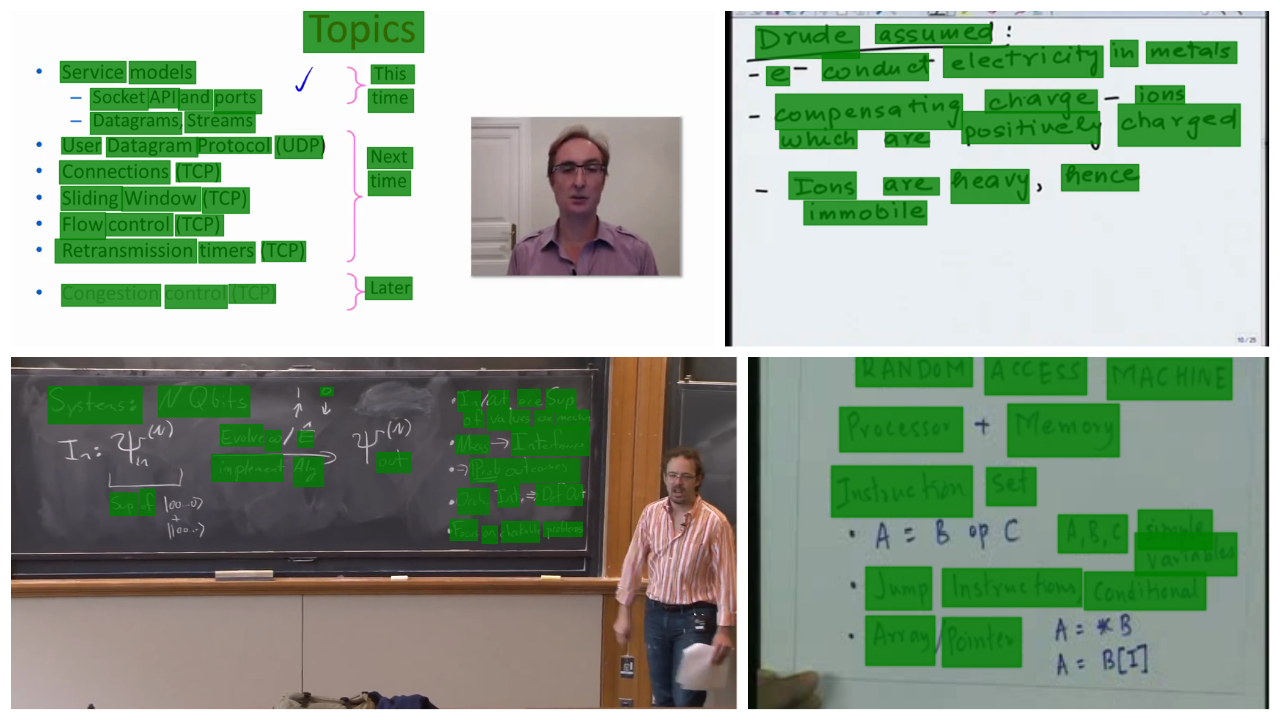
\includegraphics[width=140mm]{figures/lvdb_textdet_collage.png}
        \caption{LVDB Text Detection Samples}
        \label{meth:lvdb_textdet_collage}
\end{figure}

As most of the aforementioned models have not been explicitly trained to detect text in lecture videos, or for that matter handwritten text, and to make sure that the comparison is as fair as possible, I chose to further train (fine-tune) all of the models on the LVDB test set chosen by the dataset authors. The model fine-tuning starts based on the weights trained on the ICDAR-2015 dataset and runs for at most twenty epochs or until the performance on the validation set plateaus. The Optimizer used for training is \gls{sgd} with a $\text{momentum} = 0.9$ and $\text{weight decay} = 0.0001$ and polynomial learning rate scheduler that decreases the learning rate polynomially starting from $0.007$.

Performance metrics are the same performance metrics usually used for object detection, including precision and recall for a certain \gls{iou}, \gls{hmean}, and \gls{fps}. The \gls{iou}, also known in set theory as the Jaccard distance, is a ratio that measures how overlapping two objects or sets are. The IOU for two boxes A and B is defined as $\text{IOU} = \frac{\text{area of overlap between A and B}}{\text{area of union between A and B}}$. IOU ranges between $0$ and $1$ with a value of $1$, meaning that the two boxes overlay one another perfectly, and a value of $0$ means that the two boxes are distinct and don't overlap each other. While evaluating a model, a threshold value for the IOU can be set, so only predicted boxes that have an IOU with one of the grounded truth boxes higher than the threshold are considered. For a given IOU threshold the precision of the model's predictions can be measured, and it basically tells us how many boxes are correct out of all the predicted bounding boxes, and mathematically defined as $\text{Precision} = \nicefrac{\text{TP}}{\text{TP} + \text{FP}}$ with TP and FP being true positives and false positives correspondingly. Also, for a given IOU threshold, one can measure the Recall that indicates the percentage of the words in the picture that we found, so if there are four words in the image and we only found two, then we have a recall value of $0.5$ which is mathematically defined as $\text{Recall} = \nicefrac{\text{TP}}{\text{TP} + \text{FN}}$; with FN being the number of false negatives. If the chosen IOU threshold is $threshold$, then we denote the precision and recall measured at that threshold as Precision@$threshold$ and Recall@$threshold$; for example, for a threshold of $0.5$, we denote the measured precision and recall as Precision@.5 and Recall@.5 respectively. We also measure the precision and recall at different IOU thresholds, starting from $0.5$ and going up to $0.9$ using $0.1$ increments, and then calculate the \gls{hmean} to see how the model performs when the goal is accurate bounding boxes. Considering that these models have to be applied on hundreds of lecture video frames, they need to be as fast as possible, and a good measure of speed is the number of images processed per second denoted by \gls{fps}.

\section{Tested text recognition methods}

As is the case with text localization methods, different text recognition methods also focus on different aspects of the transcribed text. Text can vary greatly based on the used font, the person who's writing it, the language, etc thus some text recognition methods have been engineered to be better at recognizing some types of text than others. That is why we also need to do the same type of comparison of these different methods on scholarly videos. The same \gls{mmocr} framework has been selected to carry out the text recognition comparisons as it also offers implementations of multiple state-of-the-art methods.

The tested text recognition methods are \hyperref[satrn]{SATRN}, ABINet, \hyperref[master]{MASTER}, \hyperref[nrtr]{NRTR}, and \hyperref[parseq]{PARSeq}.
MMOCR had an implementation for almost all the models except for PARSeq, which I had to implement in MMOCR to measure the same performance metrics.
For more comprehensive results, the tesseract OCR engine has also been tested; it's an OCR software that was developed by HP between 1984 and 2005 when it was open-sourced and has since then been maintained by Google. It supports three OCR inference modes, called "OCR Engine modes"; mode 0 is the legacy engine mode, mode 1 is the Neural nets (LSTM) engine, and mode 3 is a combination of both modes 0 and 1.

For testing the different text recognition models a dataset and a standard set of performance metrics have been chosen. Luckily, the \gls{lvdb} dataset also contains a text recognition dataset. It has been generated by cropping out the words in the bounding boxes used for text localization and hand labeling them. The words extracted from the LVDB dataset possess the same variety as the video frames, i.e. they have different fonts, spacing, skew, weight, color, handwritten, typeset, and written by different people as shown in Figure \ref{meth:lvdb_textred_collage}.

All the tested models have been pre-trained on the SynthText \cite{gupta_synthetic_2016} and/or MJSynth \cite{jaderberg_synthetic_2014} datasets which are both synthetic datasets. These datasets are generated programmatically by overlaying random words from a dictionary over background images. SynthText contains eight million words whereas MJSynth contains nine million words. All the models were trained further on the training set of the LVDB text recognition dataset.

\begin{figure}[H]
        \centering
        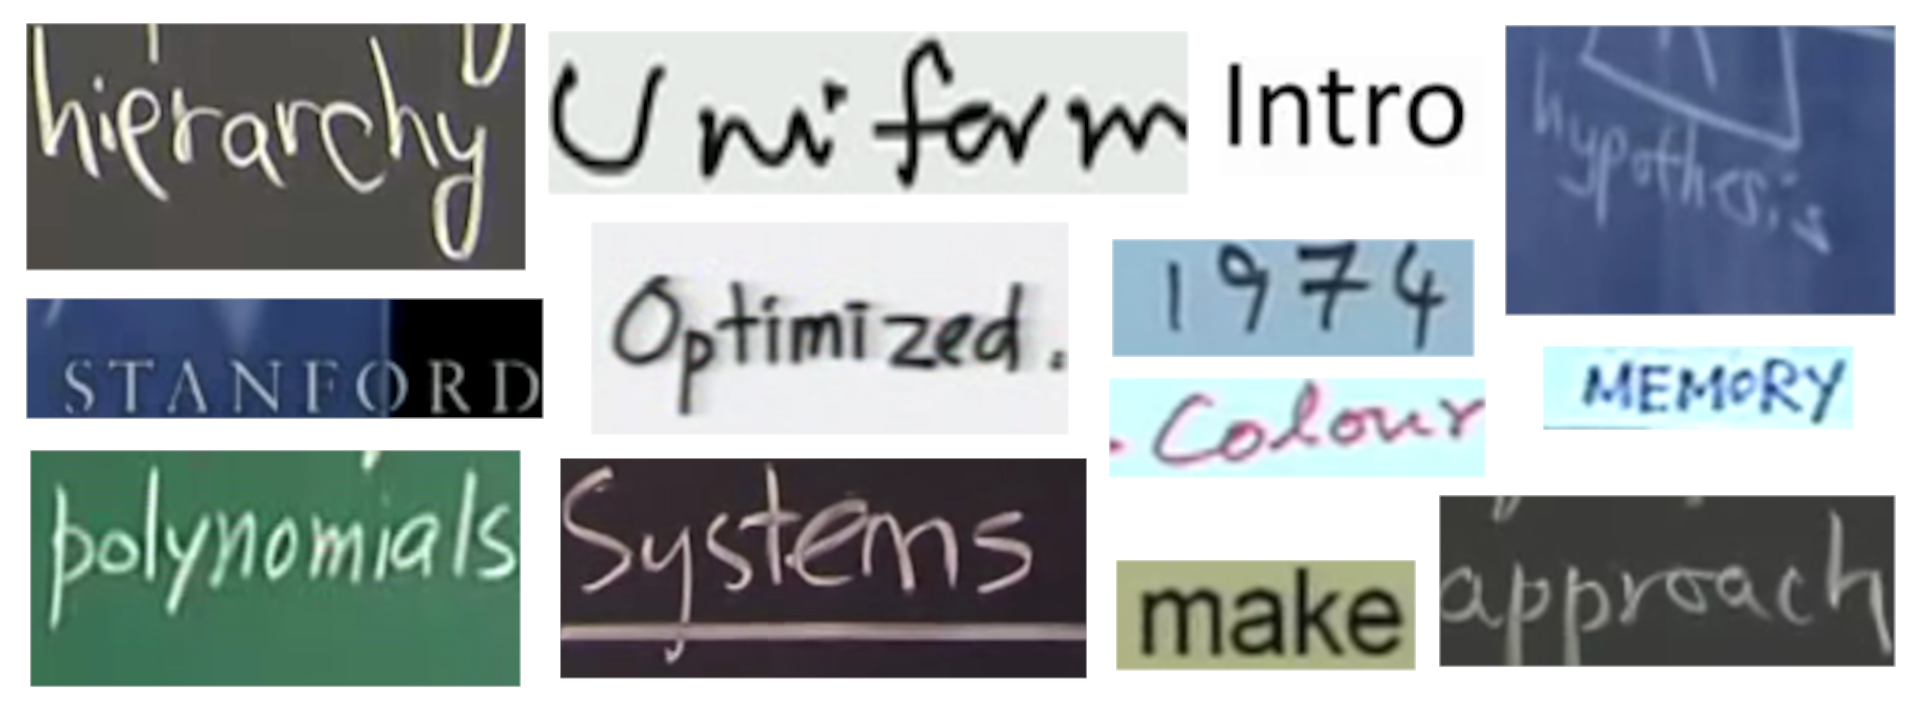
\includegraphics[width=140mm]{figures/lvdb_textrec_collage.png}
        \caption{LVDB Text Recognition Samples}
        \label{meth:lvdb_textred_collage}
\end{figure}

Text recognition methods are mainly classification models, they need object classes to transcribe. In the case of text recognition the object classes are the characters in the alphabet, we want the models to be able to recognize them. The character set chosen defines the words and hence the languages that we will be able to transcribe after the model is trained. The pre-trained models have been trained on the English alphabet (ISO basic Latin alphabet) plus punctuation characters which is also the same alphabet used by the LVDB text recognition dataset.

To determine the performance of the different models on the test set of the LVDB text recognition dataset, multiple word and character metrics have been measured. First, the word-level accuracy for all characters, without case, and without case or punctuation has been measured; it shows the percentage of the words that have been correctly transcribed while considering all the characters in the character set or only a subset of them. For example, when measuring the word accuracy without case or punctuation and our model transcribes the words "Hello!!" and "world" into "hello" and "word", then the model's accuracy is 0.5. While the word accuracy shows us the overall accuracy of the model, it fails to differentiate between a model that has extremely close results to the ground truth and a model which predicts most of the words completely wrong; consider the case in which two models A and B transcribe the word "polynomial" to "poiynomial" and "banana" respectively, they both have an accuracy of zero although model A has better/closer results to the ground truth. The \gls{1ned} metric \cite{yujian_normalized_2007} solves this problem by calculating one minus the Levenshtein edit distance between the prediction and the ground truth, so the closer the two words are the higher this metric is. For the previous example, the \gls{1ned} of "poiynomial" is $0.9$ and of "banana" is $0.19$. The model's overall \gls{1ned} is calculated for complete, uncased, and without punctuation character sets by averaging the individual word \gls{1ned}s. Added to that, the character level accuracy and recall have been measured by averaging all the characters from different words in the test set. A model might be accurate but too slow at transcribing text making its use impractical, so to make sure that the comparison is fair and to choose the best model the \gls{fps} which also represents the words per minute speed, has been taken into account.

\section{Context-free error correction}

First, to run error correction, the incorrectly transcribed (misspelled) words generated by the model have to be detected. This is usually done by verifying that the predicted word exists in a pre-defined dictionary, if it is not in the dictionary then it is considered misspelled and usually named an \gls{oov} word.
For the detection of \gls{oov} words in scholarly videos, two dictionaries have been used one for English and another for german and they were both freely available on GitHub. The English dictionary contains $466550$ words and the german dictionary contains $100000$ words. The list of the words is stored in a set (hashtable) which offers a lookup time of $O(1)$, making the \gls{oov} words detection efficient and fast.

After the misspelled words have been detected, they're passed to a context-free error correction algorithm to get suggestions for possible correction. Almost all of these methods are based on the edit distance between the predicted word and the words in the dictionary. How the distance is calculated determines the algorithm's speed and efficiency. The naive approach calculates the Levenshtein distance between the predicted word (the word to be corrected) and every word in the dictionary, sorts the words ascendingly based on the distance, and suggests the top $n$ words as corrections. This exhaustive search grows linearly with the size of the word and dictionary, and with a $400000+$ word dictionary, this quickly becomes impractical. An improvement to this method is early-stopping of the distance calculation if it exceeds a selected threshold; for a word in the dictionary, the entire distance is not calculated, only the distance up to a certain point. This method is known as "Peter Norvig"s error correction as it was proposed by him. This makes the correction faster but still too slow to be used in real-time; for example, for a word of length $n$, an alphabet size $a$ (English alphabet size), an edit distance $d$, there will be $n$ deletions, $n-1$ transpositions, $a * n$ alterations, and $a * (n+1)$ insertions, for a total of $2n+2an+a-1$ terms at search time. For $n=9$, $a=36$, $d=2$, and dictionary size of $400000+$ words this adds up to $114324 * 400000 = 45729600000$ possible terms for each \gls{oov} word, and that's only for one word but one frame of a lecture video may contain tens of words. Because of these speed limitations, the SymSpell algorithm \cite{wolf_1000x_2012} was chosen for the correction phase. In its essence, it's also somewhat similar to the naive and peter norvig's approach in that it calculates the distance between the predicted word and words in the dictionary, but completely different in the implementation. The Symspell algorithm only uses deletions to find possible corrections of the given word, and instead of calculating these deletions for every word in the dictionary during runtime, it pre-calculates and stores them in a hashmap; to find the possible corrections during runtime, it makes generates all the possible one character deletions of the word and makes a simple hashmap lookup which takes constant time. The suggestions are also based on the word frequency in the given language, which is included in the dictionary instead of the edit distance.

To measure the effectiveness of this method, the overall word accuracy with and without error correction for multiple models has been measured.

\section{Merging bonding boxes}

For merging the text into lines and paragraphs the algorithm described in \ref{ch:methodology:bouding_box_merging} has been used. It takes the list of detected and transcribed bounding boxes and creates lines out of them by first sorting the boxes based on their X and Y coordinates; it then builds the lines by putting boxes that are close enough (have X distance less than a threshold) on the same line otherwise starting a new line. This process is then done for the created lines but based on their Y distance to merge them into paragraphs. For this stage, no metrics have been measured.

\begin{algorithm}
\caption{Bounding box merging algorithm}\label{ch:methodology:bouding_box_merging}
\textbf{Input:} bboxes, max\_x\_dist, min\_x\_overlap, max\_y\_dist, min\_y\_overlap \\
\textbf{Output:} paragraphs 
\begin{algorithmic}
\State sort\_boxes\_based\_on\_y(bboxes)\;
\State stable\_sort\_boxes\_based\_on\_x(bboxes)\;
\State $\text{lines} \gets \text{[]}$
\State $\text{current\_line} \gets \text{[bboxes[0]]}$
\For{\text{bbox} \textbf{in} \text{bboxes}}
\State diff $\gets | \text{bbox.X1} - \text{current\_line.last.X2}|$
\State overlap $\gets y\_overlap(\text{bbox} , \text{current\_line.last})$
\If{diff $\ge$ max\_x\_dist \textbf{or} overlap $<$ min\_y\_overlap}
    \State lines.append(line)
    \State current\_line $\gets$ [bbox]
\EndIf
\EndFor
\State $\text{paragraphs} \gets \text{[]}$
\State $\text{current\_par} \gets \text{[lines[0]]}$
\For{\text{line} \textbf{in} \text{lines}}
\State diff $\gets | \text{line.Y1} - \text{current\_par.last.y2}|$
\State overlap $\gets x\_overlap(\text{line} , \text{current\_par})$
\If{diff $\ge$ max\_x\_dist \textbf{or} overlap $<$ min\_x\_overlap}
    \State paragraphs.append(current\_par)
    \State current\_par $\gets$ [line]
\EndIf
\EndFor
\end{algorithmic}
\end{algorithm}
\chapter{Experiments}
\chapter{Conclusion}


\singlespacing                      % References should use single
                                    % line spacing.
% \nocite{*}                        % [Debug] Use this to include all
                                    % references. 
\printbibliography                  % Print all used references.

%
\chapter{Appendix Chapter 1}

\section{Example Section for Appendix}       % Print your appendix.

\end{document}
